\documentclass[11pt]{article}
\usepackage[margin=1in]{geometry}
\usepackage{amsmath,amssymb,amsthm}
\usepackage{graphicx}
\usepackage{booktabs}
\usepackage{hyperref}
\usepackage{xcolor}
\usepackage{algorithm}
\usepackage{algorithmic}
\usepackage{subcaption}
\usepackage{enumitem}
\usepackage{multirow}

\newcommand{\R}{\mathbb{R}}
\newcommand{\norm}[1]{\|#1\|}
\newcommand{\inner}[2]{\langle #1, #2 \rangle}
\newtheorem{definition}{Definition}
\newtheorem{proposition}{Proposition}

\title{Ada-Dion V3: Per-Mode Adaptive Error Feedback\\for Communication-Efficient Spectral Optimization}

\author{
Ansh Tiwari\thanks{California Institute of Technology. \texttt{ansh@caltech.edu}}
}

\date{April 2026}

\begin{document}
\maketitle

\begin{abstract}
We present Ada-Dion V3, a communication-efficient spectral optimizer for distributed neural network training. Through a systematic experimental investigation spanning GPT-2 (45M parameters), LLaMA (300M parameters), CIFAR-10, and FashionMNIST, we identify and validate three modifications to the Dion optimizer that together yield consistent improvements. First, reducing the error-feedback coefficient to $\beta = 0.1$ provides implicit gradient memory that outperforms both standard error feedback ($\beta = 1.0$) and explicit Polyak momentum, with the improvement growing at larger model scales. Second, per-mode gradient persistence varies by a factor of $28\times$ across singular modes within a single layer, motivating per-mode adaptive feedback coefficients in place of a single scalar $\beta$. Third, through controlled experiments with QR orthogonalization, block-diagonal QR, additional power iterations, and partial orthogonalization, we find that column normalization (ColNorm) is the only right-factor method that remains stable across scales. On LLaMA 300M (WikiText-103, 15k steps), Ada-Dion V3 with adaptive rank achieves validation loss 3.403, compared to 3.565 for Dion with $\beta{=}0.3$ and 3.918 for standard Dion, while using 36\% less GPU memory. On FashionMNIST, V3 reaches 91.12\% test accuracy, compared to 90.95\% for AdamW, with $27\times$ less communication volume.
\end{abstract}

% no table of contents

% =====================================================================
\section{Introduction}
\label{sec:intro}
% =====================================================================

Training large neural networks requires distributing parameters across many GPU devices. Fully Sharded Data Parallel (FSDP)~\cite{zhao2023pytorch} is the standard approach: it partitions model parameters across devices and materializes full parameters only during the forward and backward passes through all-gather and reduce-scatter collective operations.

The choice of optimizer interacts with this sharding. Standard optimizers like AdamW~\cite{loshchilov2019decoupled} operate element-wise on gradients, so each device can update its local shard independently. Spectral optimizers like Muon~\cite{jordan2024muon}, which exploit the matrix structure of weight parameters, require the full (unsharded) gradient or momentum matrix to perform orthogonalization. This introduces additional all-gather and reduce-scatter operations that can dominate training cost at scale.

Dion~\cite{ahn2025dion} addresses this communication bottleneck by replacing Muon's full-matrix Newton-Schulz orthogonalization with a low-rank power-iteration approximation. Instead of communicating the full $m \times n$ momentum matrix, Dion communicates two factors of size $m \times r$ and $n \times r$, where $r \ll \min(m,n)$. This reduces per-step communication from $O(mn)$ to $O((m+n)r)$. To compensate for the information lost by the low-rank approximation, Dion maintains an error-feedback buffer $R_t$ that carries the residual forward to the next step.

This paper investigates three aspects of Dion's design that we find to be suboptimal in practice: the error-feedback coefficient $\beta$, the right-factor normalization, and the use of a single scalar $\beta$ across all singular modes. We describe each modification, the mathematical reasoning behind it, and the experimental evidence supporting it.

% =====================================================================
\section{Background and Notation}
\label{sec:background}
% =====================================================================

\subsection{Spectral Optimization}

Consider a matrix-shaped parameter $\theta \in \R^{m \times n}$ with loss $f(\theta)$. Standard optimizers treat $\theta$ as a flat vector and compute element-wise updates. Spectral optimizers instead seek the steepest descent direction under a matrix norm.

Concretely, the rank-$r$ steepest descent direction is defined as
\begin{equation}
\hat{D}_t = \arg\max_{\norm{D}_{(r)} \leq 1} \inner{\nabla f(\theta_t)}{D}
\label{eq:lmo}
\end{equation}
where $\norm{\cdot}_{(r)}$ denotes the dual of the Ky Fan $r$-norm. The solution is the rank-$r$ polar factor of the gradient: $\hat{D}_t = U_r V_r^\top$, where $U_r, V_r$ are the top-$r$ left and right singular vectors of $\nabla f(\theta_t)$.

Computing this exactly requires an SVD at cost $O(mn \cdot \min(m,n))$, which is too expensive for large matrices. Muon approximates it via Newton-Schulz iteration on the full momentum matrix. Dion approximates it via one step of subspace iteration on a rank-$r$ factorization.

\subsection{The Dion Algorithm}

\begin{definition}[Dion optimizer]
At each step $t$, Dion maintains a momentum/error buffer $R_t \in \R^{m \times n}$ and a warm-start matrix $V_{t-1} \in \R^{n \times r}$. The update proceeds as:
\begin{enumerate}[nosep]
    \item Form the effective gradient: $M_t = G_t + R_t$, where $G_t = \nabla f(\theta_t)$.
    \item Power iteration: $U_t = \mathrm{orth}(M_t V_{t-1})$, producing $U_t \in \R^{m \times r}$ with orthonormal columns.
    \item Compute the right factor: $W_t = M_t^\top U_t \in \R^{n \times r}$.
    \item Normalize: $\bar{V}_t = \mathrm{ColNorm}(W_t)$, where $\mathrm{ColNorm}$ divides each column by its $\ell_2$ norm.
    \item Update parameters: $\theta_{t+1} = \theta_t - \eta \, U_t \bar{V}_t^\top$.
    \item Error feedback: $R_{t+1} = M_t - \beta \, U_t U_t^\top M_t$.
\end{enumerate}
\end{definition}

The error-feedback step (6) decomposes naturally. Let $P_t = U_t U_t^\top$ denote the tracked rank-$r$ projector. Then
\begin{equation}
R_{t+1} = \underbrace{(I - P_t) M_t}_{\text{structural tail}} + \underbrace{(1-\beta) \, P_t M_t}_{\text{retained signal}}
\label{eq:ef_decomp}
\end{equation}
The structural tail $(I - P_t) M_t$ is the part of $M_t$ that lies outside the rank-$r$ subspace and would be lost without error feedback. With $\beta = 1$ (standard Dion), the retained signal vanishes and $R_{t+1}$ contains only the structural tail. With $\beta < 1$, a fraction $(1-\beta)$ of the captured signal is deliberately kept in the buffer.

\subsection{The One-Step Descent Bound}

The convergence analysis of Dion-family optimizers rests on a descent lemma. Under a non-Euclidean smoothness assumption (Assumption A in~\cite{ahn2025dion}), the one-step progress satisfies
\begin{equation}
f(\theta_{t+1}) \leq f(\theta_t) - \eta \norm{G_t}_{\mathrm{KF},r} + \eta\big(\delta_t + (1 + \nu_t)\norm{R_t}_{\mathrm{KF},r}\big) + \frac{L_r \nu_t^2}{2}\eta^2
\label{eq:descent}
\end{equation}
where:
\begin{itemize}[nosep]
    \item $\norm{G_t}_{\mathrm{KF},r} = \sum_{i=1}^r \sigma_i(G_t)$ is the Ky Fan $r$-norm (sum of top-$r$ singular values).
    \item $\delta_t = \norm{M_t}_{\mathrm{KF},r} - \inner{M_t}{\hat{D}_t}$ is the oracle defect, measuring how far the actual update is from the optimal rank-$r$ direction.
    \item $\nu_t = \norm{\hat{D}_t}_{(r)}$ is the dual Ky Fan norm of the update direction. For a partial isometry (all singular values 0 or 1), $\nu_t = 1$. For ColNorm output, $\nu_t$ can be as large as $\sqrt{r}$.
    \item $L_r$ is the non-Euclidean smoothness constant.
\end{itemize}

Two terms in~\eqref{eq:descent} involve $\nu_t$: the residual coupling $(1+\nu_t)\norm{R_t}$ and the smoothness penalty $L_r \nu_t^2 \eta^2 / 2$. The smoothness penalty appears quadratically in $\nu_t$, so reducing $\nu_t$ from $\sqrt{r}$ to $1$ would reduce this term by a factor of $r$. This observation motivates the Orth-Dion proposal (replacing ColNorm with QR), which we investigate in Section~\ref{sec:qr}.

\subsection{Effective Rank}

\begin{definition}[Effective rank]
Given a matrix $M$ with singular values $\sigma_1 \geq \sigma_2 \geq \cdots$, the effective rank is
\[
\mathrm{erank}(M) = \exp\Big(-\sum_i p_i \log p_i\Big), \quad p_i = \frac{\sigma_i}{\sum_j \sigma_j}.
\]
\end{definition}
The effective rank is a continuous measure of the number of significant singular directions. It equals $k$ exactly when all $k$ singular values are equal and the rest are zero. In practice, it lies between 1 (one dominant direction) and $\min(m,n)$ (uniform spectrum). We use column norms of $W_t = M_t^\top U_t$ as proxy singular values.

\subsection{The Three Regimes of Error Feedback}
\label{sec:three_regimes}

To understand the role of $\beta$, we need the concept of gradient subspace persistence, which characterizes how the out-of-subspace gradient components evolve across steps.

\begin{definition}[Gradient subspace persistence]
Let $P_t = U_t U_t^\top$ be the tracked projector at step $t$. The out-of-subspace gradient component is $(I - P_t) G_t$. The persistence at step $t$ is
\[
\rho_t = \frac{\inner{(I-P_t)G_t}{(I-P_{t-1})G_{t-1}}}{\norm{(I-P_t)G_t} \cdot \norm{(I-P_{t-1})G_{t-1}}}
\]
which is the cosine similarity between consecutive out-of-subspace gradient components.
\end{definition}

The value of $\rho_t$ determines whether the error-feedback buffer helps or hurts. There are three qualitatively different regimes:

\paragraph{Regime 1: Coherent accumulation ($\rho_t > 0$).} When the out-of-subspace gradient components point in a consistent direction across steps, the error-feedback buffer accumulates a coherent signal. Unrolling the recursion,
\[
R_T \approx \sum_{t=0}^{T-1} (I - P_t) G_t.
\]
The terms add constructively rather than cancelling. When the tracked subspace eventually rotates to capture this direction, the buffer delivers a large, useful correction. In this regime, $\beta = 1$ is optimal because it preserves the structural tail faithfully without adding noise from the retained signal.

A synthetic experiment with controlled persistent gradient directions ($\rho_t \approx 0.58$) confirms this: error feedback on yields final loss $1.86 \times 10^{-4}$, while error feedback off yields $38.9$, a ratio of approximately $200{,}000\times$.

\paragraph{Regime 2: Implicit momentum ($\rho_t \approx 0$).} When out-of-subspace components are approximately independent across steps, the buffer performs a random walk with magnitude $\norm{R_T}_F \sim \sqrt{T} \cdot \hat{\epsilon}_t \cdot \norm{G}_F$, where $\hat{\epsilon}_t = \norm{(I-P_t)M_t}_F / \norm{M_t}_F$ is the tracking error.

Although the directions are random, the buffer still provides useful signal. Specifically, when the tracked subspace rotates slowly, the buffer acts as an implicit momentum term. If the subspace rotates at rate $\theta$ per step, the expected recovered signal satisfies
\[
\mathbb{E}[P_{T} R_T] \approx \hat{\epsilon}_t^2 \cdot \sum_{t < T} \gamma(\theta)^{T-t} \nabla f(\theta_t)
\]
for an effective decay coefficient $\gamma(\theta) = 1 - O(\theta^2)$ determined by the rotation rate. This is a heavy-ball momentum term with effective coefficient $\hat{\epsilon}_t^2$.

For ColNorm (where $\hat{\epsilon}_t \approx 0.15$--$0.30$), this implicit momentum coefficient is $0.02$--$0.09$, which is small but nonzero. For QR (where $\hat{\epsilon}_t \approx 0.007$), it is approximately $5 \times 10^{-5}$, which is negligible. This difference is central to understanding why QR fails in practice (Section~\ref{sec:qr}).

In this regime, $\beta < 1$ is beneficial because it increases $\norm{R_t}$ and thereby amplifies the implicit momentum effect. The optimal $\beta$ balances signal accumulation against noise growth. Empirically, $\beta \approx 0.1$--$0.3$ works best.

\paragraph{Regime 3: Divergence ($\rho_t < 0$).} When out-of-subspace components anti-correlate across steps, the buffer accumulates noise that the subspace cannot absorb. The buffer grows without bound and error feedback becomes harmful. In this regime, $\beta$ should be set close to 0.

A synthetic experiment with rotating gradient directions ($\rho_t \approx 0.05$) confirms this: error feedback on yields final loss 34.8, while error feedback off yields 33.0. Error feedback hurts by 5\%.

\paragraph{Generic LLM training falls in Regime 2.} Measurements on WikiText-103 with GPT-2 45M show $\rho_t \approx -0.01$ (near zero, slightly negative), placing standard LLM training in or near Regime~2. This explains why $\beta < 1$ consistently helps: the implicit momentum mechanism is active, and reducing $\beta$ amplifies it.

\subsection{The Residual Decomposition}

To formalize the analysis, we decompose the error-feedback residual into three components. Let $P_t^* = U_{r,t} U_{r,t}^\top$ denote the exact top-$r$ projector of $M_t$ (from SVD). Then

\begin{equation}
R_{t+1} = \underbrace{(I - P_t^*) M_t}_{T_t^* \text{ (structural tail)}} + \underbrace{(P_t^* - P_t) M_t}_{E_t \text{ (tracking defect)}} + \underbrace{(1-\beta_t) P_t M_t}_{S_t \text{ (persistence term)}}
\label{eq:residual_decomp}
\end{equation}

The structural tail $T_t^*$ is not an optimizer failure; it is the unavoidable residual left by any rank-$r$ method. The tracking defect $E_t$ is the true algorithmic error, which should be $O(\eta)$ under good tracking conditions. The persistence term $S_t$ is the deliberate memory channel created by $\beta < 1$.

Standard Dion ($\beta = 1$) sets $S_t = 0$, leaving $R_{t+1} = T_t^* + E_t$. Ada-Dion V3 ($\beta < 1$, per-mode) controls the persistence term on a per-mode basis.

% =====================================================================
\section{The Ada-Dion V3 Algorithm}
\label{sec:algorithm}
% =====================================================================

Ada-Dion V3 modifies Dion in three ways: (1) the scalar $\beta$ is replaced by a per-mode vector $b = (b_1, \ldots, b_r)$, (2) the base retention level is set to $\beta_0 = 0.1$ rather than 1.0, and (3) adaptive rank selection is optionally enabled. The right-factor normalization remains ColNorm.

% Color legend for algorithm:
%   Black  = inherited from Dion (base algorithm)
%   Green  = from Ada-Dion V2 (adaptive rank, modified feedback coefficient)
%   Red    = new in Ada-Dion V3 (per-mode persistence, buffer ceiling)
\definecolor{v2green}{RGB}{0,130,30}
\definecolor{v3red}{RGB}{190,30,30}

\begin{algorithm}[H]
\caption{Ada-Dion V3. {\normalfont Black: inherited from Dion. {\color{v2green}Green}: from Ada-Dion V2. {\color{v3red}Red}: new in Ada-Dion V3.}}
\label{alg:adadion_v3}
\begin{algorithmic}[1]
\REQUIRE learning rate $\eta$, rank $r$, {\color{v2green}base coefficient $\beta_0 = 0.1$}, {\color{v3red}sigmoid sharpness $s = 10$}
\REQUIRE {\color{v3red}EMA decay $\alpha = 0.95$, buffer ceiling $R_{\max} = 5.0$}
\STATE Initialize $R_0 = 0$, $V_0 = \mathrm{orth}(\mathrm{randn}(n, r))$, {\color{v3red}$\bar{\rho}_{i,0} = 0$ for $i = 1, \ldots, r$}
\FOR{$t = 1, 2, \ldots, T$}

    \STATE $M_t \gets G_t + R_t$ \hfill \COMMENT{effective gradient}

    \STATE $U_t \gets \mathrm{orth}(M_t V_{t-1})$ \hfill \COMMENT{power iteration, left factor}
    \STATE $W_t \gets M_t^\top U_t$ \hfill \COMMENT{unnormalized right factor}
    \STATE $\bar{V}_t \gets \mathrm{ColNorm}(W_t)$ \hfill \COMMENT{column normalization}

    \STATE $\theta_{t+1} \gets \theta_t - \eta \, U_t \bar{V}_t^\top$ \hfill \COMMENT{rank-$r$ update}

    \FOR{{\color{v3red}$i = 1, \ldots, r$}} \COMMENT{{\color{v3red}per-mode gradient persistence (V3)}}
        \STATE {\color{v3red}$\rho_{i,t} \gets \mathrm{cos\_sim}(U_t\lbrack :,i\rbrack^\top G_t, \; U_t\lbrack :,i\rbrack^\top G_{t-1})$} \hfill \COMMENT{{\color{v3red}cosine similarity}}
        \STATE {\color{v3red}$\bar{\rho}_{i,t} \gets \alpha \, \bar{\rho}_{i,t-1} + (1 - \alpha) \, \rho_{i,t}$} \hfill \COMMENT{{\color{v3red}EMA smoothing}}
    \ENDFOR

    \STATE {\color{v3red}$b_i \gets \sigma(s \cdot \bar{\rho}_{i,t})$ for $i = 1,\ldots,r$} \hfill \COMMENT{{\color{v3red}per-mode feedback coefficient}}
    \STATE {\color{v3red}$b_i \gets b_i \cdot \beta_0 / \mathrm{mean}(b)$} \hfill \COMMENT{{\color{v3red}rescale to target mean $\beta_0$}}
    \STATE {\color{v3red}$b_i \gets \mathrm{clamp}(b_i, 0.05, 0.95)$}

    \STATE {\color{v2green}$R_{t+1} \gets M_t - U_t \, \mathrm{diag}(b_1, \ldots, b_r) \, U_t^\top M_t$} \hfill \COMMENT{{\color{v2green}modified error feedback}}

    \IF{{\color{v3red}$\norm{R_{t+1}}_F / \norm{G_t}_F > R_{\max}$}}
        \STATE {\color{v3red}$R_{t+1} \gets R_{t+1} \cdot R_{\max} \norm{G_t}_F / \norm{R_{t+1}}_F$} \hfill \COMMENT{{\color{v3red}buffer ceiling (V3)}}
    \ENDIF

    \STATE $V_t \gets \mathrm{ColNorm}(W_t)$ \hfill \COMMENT{warm-start for next step}

    \STATE {\color{v2green}\textit{(Optional) Adaptive rank: adjust $r$ via effective rank of $W_t$}} \hfill \COMMENT{{\color{v2green}from V2}}

\ENDFOR
\end{algorithmic}
\end{algorithm}

\subsection{Per-Mode Feedback: Mathematical Rationale}

The per-mode feedback coefficient $b_i$ for mode $i$ is determined by the EMA-smoothed persistence $\bar{\rho}_{i,t}$ through a sigmoid:
\[
b_i = \sigma(s \cdot \bar{\rho}_{i,t}) = \frac{1}{1 + e^{-s \bar{\rho}_{i,t}}}
\]
This mapping has two desirable properties. First, modes with high persistence ($\bar{\rho}_{i,t} \gg 0$, Regime~1 behavior) get $b_i \to 1$, meaning their captured signal is cleared and the structural tail is preserved faithfully. Second, modes with low or negative persistence ($\bar{\rho}_{i,t} \leq 0$, Regime~2 or~3 behavior) get $b_i \to 0$, meaning most of the captured signal is retained as memory. The rescaling step ensures $\mathrm{mean}(b) \approx \beta_0$, so the average retention level matches the target.

\subsection{Buffer Ceiling: Mathematical Rationale}

With $\beta_0 = 0.1$, each step retains approximately 90\% of the captured signal. Without a ceiling, $\norm{R_t}$ grows roughly as
\[
\norm{R_t}_F \approx \frac{1 - (1-\hat{\epsilon}_t)^t}{\hat{\epsilon}_t} \cdot \norm{G}_F
\]
where $\hat{\epsilon}_t$ is the tracking error. For $\hat{\epsilon}_t \approx 0.15$ and $t = 100$ steps, this gives $\norm{R_t} / \norm{G} \approx 6.5$. The response surface analysis (Section~\ref{sec:response}) shows that the optimal buffer-to-gradient ratio is $\lambda^* \approx 1.0$--$1.3$, so allowing $R_{\mathrm{norm}}$ to grow to 6.5 is suboptimal. The ceiling $R_{\max} = 5.0$ provides headroom while preventing excessive growth.

\subsection{Communication Cost}

The per-step communication is identical to Dion: $O((m+n) \cdot r)$ floats per matrix parameter. All V3-specific computations (per-mode $\rho_i$, sigmoid, buffer clamping) are local operations on each device and require no communication.

\subsection{Parameter Routing}

Not all parameters benefit from spectral updates. Embedding matrices (e.g., $50{,}257 \times d$) are lookup tables with no natural low-rank structure. One-dimensional parameters (layer norms, biases) have no matrix structure. V3 routes these to an internal AdamW optimizer at learning rate $3 \times 10^{-4}$. The spectral update is applied only to weight matrices with aspect ratio $\max(m,n) / \min(m,n) \leq 16$ and $\min(m,n) \geq r$.

% =====================================================================
\section{Experiment 1: Buffer Retention ($\beta < 1$)}
\label{sec:beta}
% =====================================================================

\subsection{Setup}

We train GPT-2 (45M parameters, 6 layers, 512 hidden, 8 heads) on WikiText-103 for 30{,}000 steps with $r = 64$, batch size 8, sequence length 1024, cosine learning rate schedule (peak $\eta = 0.01$, warmup 3000 steps, minimum ratio 0.1), weight decay 0.1, and gradient clipping at norm 1.0. We sweep $\beta \in \{0.0, 0.3, 0.5, 0.7, 1.0\}$, holding all other hyperparameters fixed.

\subsection{Results}

\begin{figure}[h]
\centering
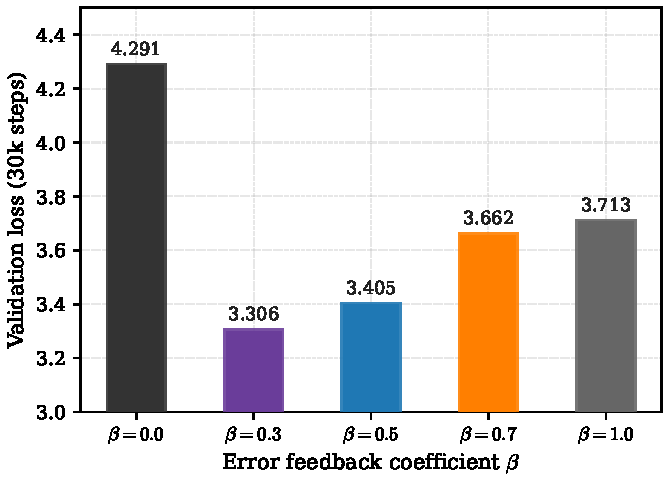
\includegraphics[width=0.55\linewidth]{figs/fig7_beta_sweep.pdf}
\caption{Validation loss vs.\ $\beta$ (GPT-2 45M, WikiText-103, 30k steps). Every $\beta < 1$ outperforms the standard $\beta = 1$ baseline. The improvement is monotone. $\beta = 0$ (no error feedback) is the worst.}
\label{fig:beta_sweep}
\end{figure}

\begin{table}[h]
\centering
\caption{$\beta$ sweep results (GPT-2 45M, WikiText-103, 30k steps, $r{=}64$).}
\label{tab:beta_sweep}
\begin{tabular}{lcc}
\toprule
\textbf{Method} & \textbf{Val Loss} & \textbf{vs.\ $\beta = 1$} \\
\midrule
Flat $\beta = 0.3$ & 3.306 & $-0.407$ \\
Flat $\beta = 0.5$ & 3.405 & $-0.307$ \\
Flat $\beta = 0.7$ & 3.662 & $-0.051$ \\
Dion $\beta = 1.0$ (baseline) & 3.713 & -- \\
No EF ($\beta = 0$) & 4.291 & $+0.578$ \\
\bottomrule
\end{tabular}
\end{table}

The ordering is $\beta{=}0.3 < \beta{=}0.5 < \beta{=}0.7 < \beta{=}1.0 < \beta{=}0.0$, with the best result ($\beta = 0.3$) improving over the baseline by 0.407 nats at zero additional compute cost. The no-EF variant ($\beta = 0$) is 0.578 nats worse than $\beta = 1$, confirming that error feedback is essential; the question is how much captured signal to retain.

\subsection{Rank Interaction}

The $\beta < 1$ benefit persists at every rank tested ($r \in \{8, 16, 32, 128, 256\}$), with a gap of 0.18--0.29 nats between $\beta = 0.3$ and $\beta = 1.0$ (Figure~\ref{fig:rank_beta}). This rules out the hypothesis that $\beta < 1$ only helps when the rank is insufficient, as it provides a consistent gain regardless of rank.

\begin{figure}[h]
\centering
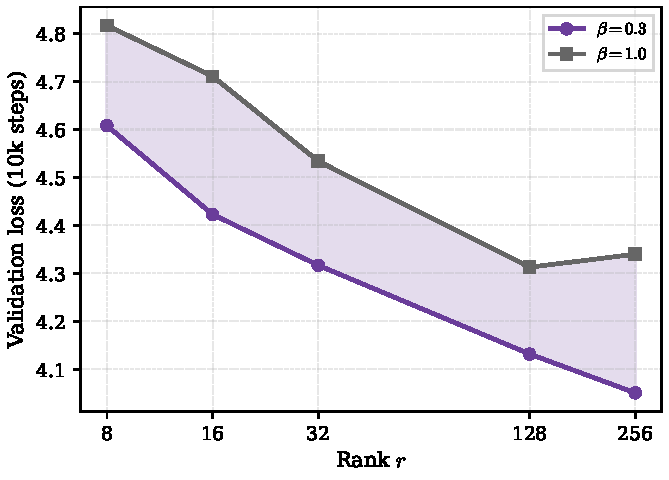
\includegraphics[width=0.55\linewidth]{figs/fig8_rank_beta.pdf}
\caption{Validation loss vs.\ rank for $\beta = 0.3$ (purple) and $\beta = 1.0$ (gray). The gap is consistent at 0.18--0.29 nats across all ranks.}
\label{fig:rank_beta}
\end{figure}

\subsection{Buffer Retention vs.\ Polyak Momentum}

To distinguish the implicit momentum mechanism from standard gradient averaging, we compare against PolyakDion: explicit Polyak heavy-ball momentum ($m_t = 0.95 \cdot m_{t-1} + 0.05 \cdot G_t$) with the rank-$r$ update applied to $m_t$, and $R \equiv 0$ (no error-feedback buffer). This isolates the question: does the buffer's interaction with the rank-$r$ compression provide something beyond simple momentum?

PolyakDion achieves val loss 3.459, compared to 3.306 for $\beta = 0.3$. The 0.153 nat gap indicates that the buffer mechanism is distinct from standard momentum. The difference arises because the buffer reshapes the input $M_t = G_t + R_t$ to the power iteration step, changing which subspace is tracked. Polyak momentum averages gradients before compression and does not affect subspace selection in the same way.

% =====================================================================
\section{Experiment 2: QR Failure Investigation}
\label{sec:qr}
% =====================================================================

\subsection{Theoretical Motivation}

The Orth-Dion convergence analysis~\cite{ahn2025dion} replaces ColNorm with QR factorization in the right factor, guaranteeing $\nu_t = 1$ (since $U_t \bar{V}_t^\top$ becomes a partial isometry with all singular values 0 or 1). This eliminates the $\sqrt{r}$ factor from the convergence rate's leading constant:
\[
\text{ColNorm: } O\!\left(\sqrt{\frac{L_r \cdot r}{T}}\right), \qquad \text{QR: } O\!\left(\sqrt{\frac{L_r}{T}}\right).
\]
At $r = 64$, this predicts an $8\times$ improvement in the convergence constant.

\subsection{Experimental Design}

We test this prediction with 16 controlled experiments on GPT-2 45M (WikiText-103, 10k steps):
\begin{itemize}[nosep]
    \item ColNorm and QR at ranks $r \in \{8, 16, 32, 64\}$ (8 experiments).
    \item QR with 3 power iterations instead of 1 (1 experiment).
    \item Block-diagonal QR with block sizes $k \in \{4, 8, 16\}$ (3 experiments).
    \item Partial orthogonalization with 1 and 2 correction rounds (2 experiments).
    \item Exact truncated SVD as gold standard (1 experiment).
    \item ColNorm for 5000 steps then switch to QR (1 experiment).
\end{itemize}

\subsection{QR Fails at All Ranks}

\begin{figure}[h]
\centering
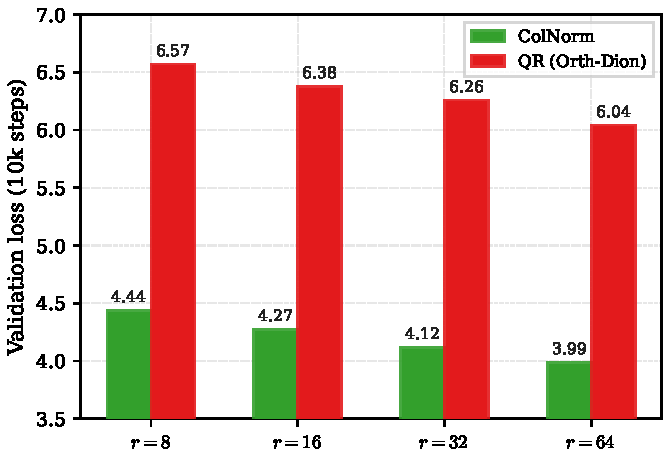
\includegraphics[width=0.55\linewidth]{figs/fig4_qr_vs_colnorm.pdf}
\caption{ColNorm vs.\ QR at ranks $r = 8, 16, 32, 64$. QR produces 2+ nats worse validation loss at every rank. There is no crossover.}
\label{fig:qr_vs_colnorm}
\end{figure}

Figure~\ref{fig:qr_vs_colnorm} shows that QR fails at every rank tested. The gap is approximately 2 nats throughout, with no trend suggesting convergence at higher or lower ranks. This indicates that the failure is not due to insufficient rank.

\subsection{Comprehensive Right-Factor Comparison}

\begin{figure}[h]
\centering
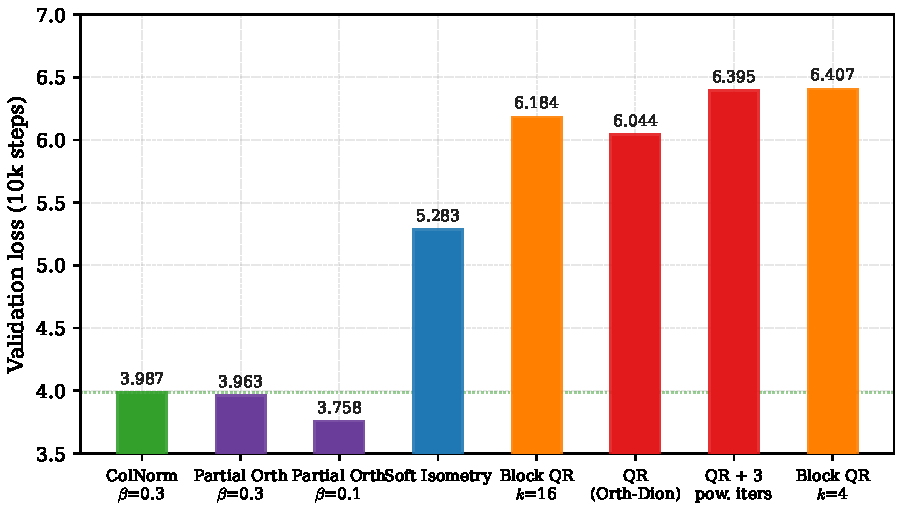
\includegraphics[width=0.75\linewidth]{figs/fig5_right_factor.pdf}
\caption{All right-factor methods. Any form of inter-column orthogonalization (full QR, block QR, QR with multiple power iterations) results in validation loss above 6.0. ColNorm remains stable at 3.99.}
\label{fig:right_factor}
\end{figure}

\subsection{Root Cause Analysis}

We collect per-parameter diagnostics at step 15{,}000 (Figure~\ref{fig:diagnostics}) comparing ColNorm, QR, and Soft Isometry.

\begin{figure}[h]
\centering
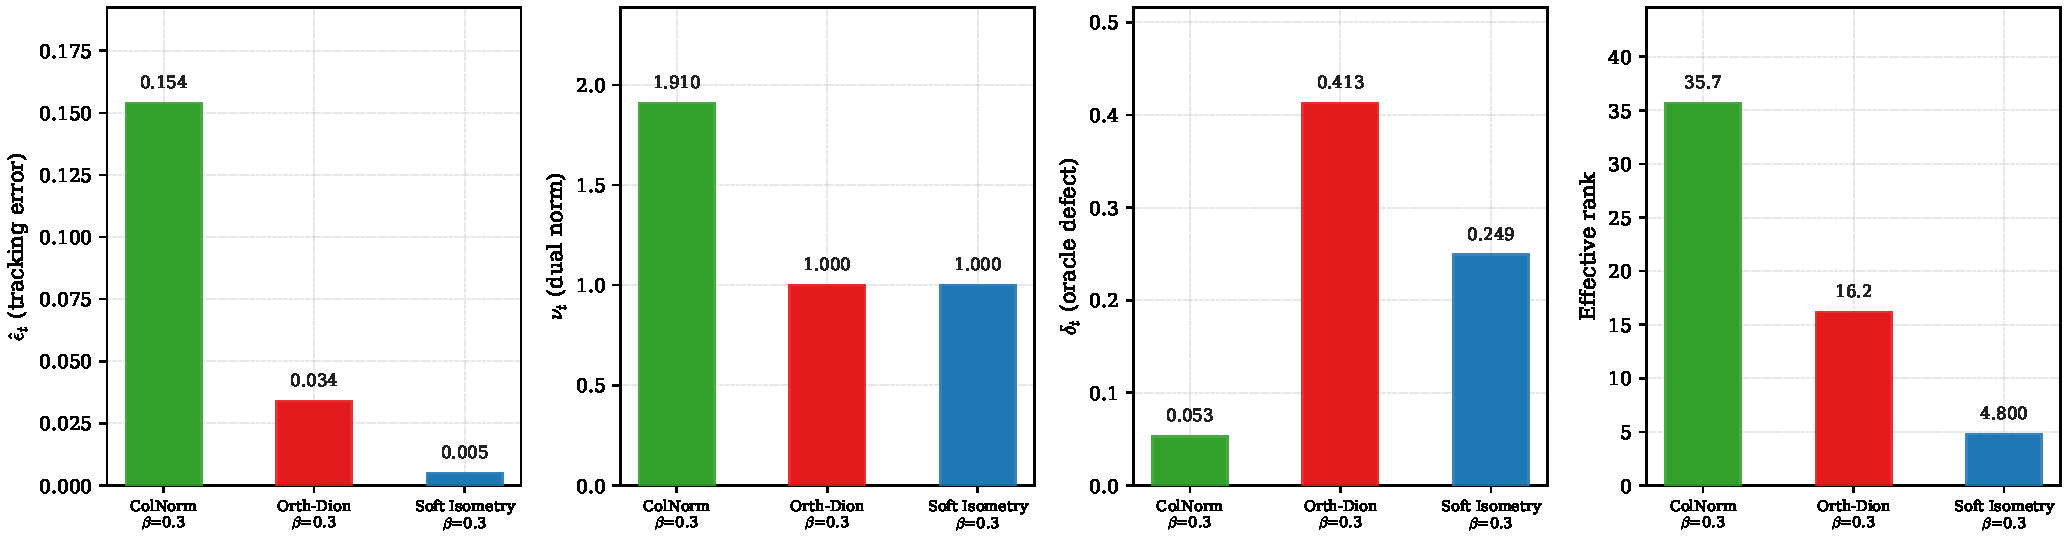
\includegraphics[width=\linewidth]{figs/fig6_diagnostics.pdf}
\caption{Four diagnostic quantities at step 15{,}000 for three right-factor methods. QR achieves $\nu_t = 1$ but collapses effective rank to 16.2 (from ColNorm's 35.7) and increases $\delta_t$ by $8\times$.}
\label{fig:diagnostics}
\end{figure}

The diagnostics reveal the failure mechanism. QR achieves $\nu_t = 1.00$ as theory predicts, but this comes at the cost of effective rank collapse (from 35.7 to 16.2) and an $8\times$ increase in the oracle defect $\delta_t$ (from 0.053 to 0.413).

\paragraph{Why the defect dominates.} Substituting into the descent bound~\eqref{eq:descent} with $\eta = 0.01$:
\begin{align*}
\text{ColNorm: } &\quad -\eta \delta_t = -0.01 \times 0.053 = -5.3 \times 10^{-4}, \quad \frac{L_r \nu_t^2 \eta^2}{2} = \frac{L_r \times 3.64 \times 10^{-4}}{2} \\
\text{QR: } &\quad -\eta \delta_t = -0.01 \times 0.413 = -4.1 \times 10^{-3}, \quad \frac{L_r \nu_t^2 \eta^2}{2} = \frac{L_r \times 10^{-4}}{2}
\end{align*}
QR loses $3.6 \times 10^{-3}$ per step from the larger defect and gains at most $L_r \times 1.3 \times 10^{-4}$ from the smaller $\nu_t$. Even at $L_r = 1$, the defect cost is $28\times$ larger than the $\nu_t$ benefit.

\paragraph{Why QR collapses effective rank.} QR performs Gram-Schmidt orthogonalization on $W = M_t^\top U$. When the column norms of $W$ span several orders of magnitude (which occurs generically when the spectral ratio $\sigma_{r+1}/\sigma_r \approx 0.98$), Gram-Schmidt forces later columns to be orthogonal to dominant early columns. This pushes weak but real singular directions toward noise. ColNorm normalizes each column independently, preserving all $r$ directions regardless of their relative magnitude.

Mathematically, the descent-relevant inner product satisfies
\begin{align}
\text{ColNorm:} \quad \inner{M}{\hat{D}} &= \sum_{j=1}^r \norm{w_j}_2 \label{eq:cn_inner} \\
\text{QR:} \quad \inner{M}{\hat{D}} &= \mathrm{tr}(R) = \sum_{j=1}^r R_{jj} \leq \sum_{j=1}^r \norm{w_j}_2 \label{eq:qr_inner}
\end{align}
where $R$ is the upper triangular factor from $W = QR$. The inequality~\eqref{eq:qr_inner} is strict whenever columns of $W$ are correlated.

\paragraph{Additional negative results.}
\begin{itemize}[nosep]
    \item \textbf{More power iterations do not help.} QR with 3 power iterations (6.395) is no better than QR with 1 (6.044). The problem is in the right-factor normalization, not the left-factor quality.
    \item \textbf{Block-diagonal QR also fails.} Even orthogonalizing within blocks of 4 columns (block QR $k{=}4$: 6.407) is sufficient to degrade training to near-QR levels.
    \item \textbf{ColNorm-to-QR switching fails.} Starting with ColNorm for 5000 steps then switching to QR produces val loss 5.457. This indicates QR failure is not an initialization problem.
    \item \textbf{Exact SVD performs best.} Truncated SVD (3.946) slightly outperforms ColNorm (3.987), confirming that perfect subspace tracking helps. The 0.041 nat gap represents the ceiling for any power-iteration-based method.
\end{itemize}

\paragraph{Connection to the three-regime framework.} QR's failure can be understood through the implicit momentum mechanism described in Section~\ref{sec:three_regimes}. QR produces tracking error $\hat{\epsilon}_t \approx 0.007$, compared to ColNorm's $\hat{\epsilon}_t \approx 0.15$--$0.30$. Since the implicit momentum coefficient scales as $\hat{\epsilon}_t^2$, QR reduces it from $\sim$$0.04$ to $\sim$$5 \times 10^{-5}$. In Regime~2 (generic LLM training), this eliminates the buffer retention mechanism that makes $\beta < 1$ effective. The right-factor geometry and buffer retention are coupled, not independent design axes.

% =====================================================================
\section{Experiment 3: Per-Mode Persistence Heterogeneity}
\label{sec:modewise}
% =====================================================================

The three-regime analysis in Section~\ref{sec:three_regimes} uses a single scalar $\rho_t$ to characterize gradient persistence. But the effective gradient $M_t$ is a matrix with $r$ tracked singular modes, and each mode may have different persistence characteristics. If some modes are in Regime~1 while others are in Regime~2 or~3, a scalar $\beta$ cannot serve all of them.

We measure per-mode persistence $\rho_{i,t}$ for each of the $r = 64$ modes during training of GPT-2 45M on WikiText-103 ($\beta = 0.3$, 10k steps, diagnostics every 50 steps).

\begin{figure}[h]
\centering
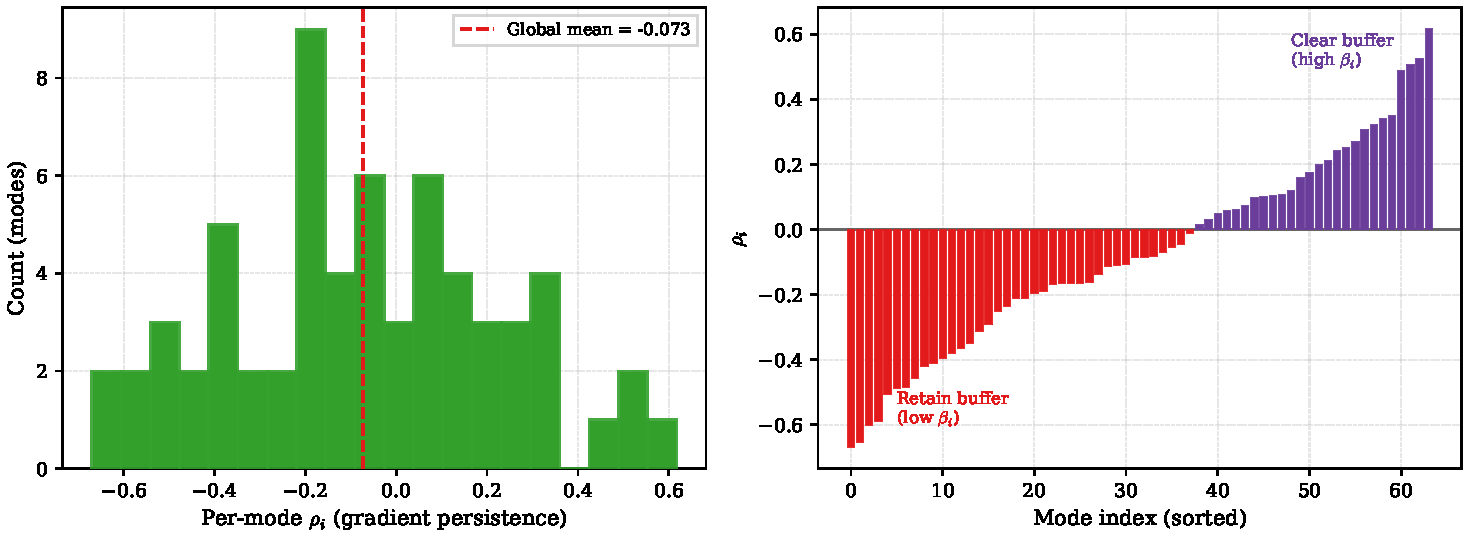
\includegraphics[width=0.85\linewidth]{figs/fig9_modewise.pdf}
\caption{(Left) Distribution of per-mode $\rho_i$ across 64 modes in late training (steps 5k--10k). The global mean is $-0.008$, but individual modes range from $-0.5$ to $+0.5$. (Right) Per-mode $\rho_i$ sorted by value. Purple indicates modes that would benefit from high $b_i$ (clear buffer); red indicates modes that would benefit from low $b_i$ (retain buffer).}
\label{fig:modewise}
\end{figure}

\begin{table}[h]
\centering
\caption{Per-mode persistence statistics (late training, steps 5{,}000--10{,}000, $r{=}64$).}
\label{tab:modewise}
\begin{tabular}{lc}
\toprule
\textbf{Statistic} & \textbf{Value} \\
\midrule
Mean $\rho_i$ across modes & $-0.008$ \\
Std $\rho_i$ across modes & $0.338$ \\
Heterogeneity (std / $|\mathrm{mean}|$) & $28.4\times$ \\
Std of per-mode $u_i$ (re-entry) & $0.053$ \\
\bottomrule
\end{tabular}
\end{table}

The heterogeneity ratio of $28.4\times$ (standard deviation is 28 times the absolute mean) indicates that modes have very different persistence characteristics. A scalar $\beta$ sees the near-zero global mean and applies the same retention to all modes. Per-mode control can apply high $b_i$ (clear buffer) to modes with $\rho_i > 0$ and low $b_i$ (retain buffer) to modes with $\rho_i < 0$.

% =====================================================================
\section{Experiment 4: Response Surface Analysis}
\label{sec:response}
% =====================================================================

To understand the optimal buffer size, we freeze checkpoints from completed training runs and measure the one-step loss change when scaling the buffer: $M(\lambda) = G + \lambda R$, for $\lambda \in \{0, 0.25, 0.5, \ldots, 5.0\}$. Results are averaged over 10 batches.

\begin{figure}[h]
\centering
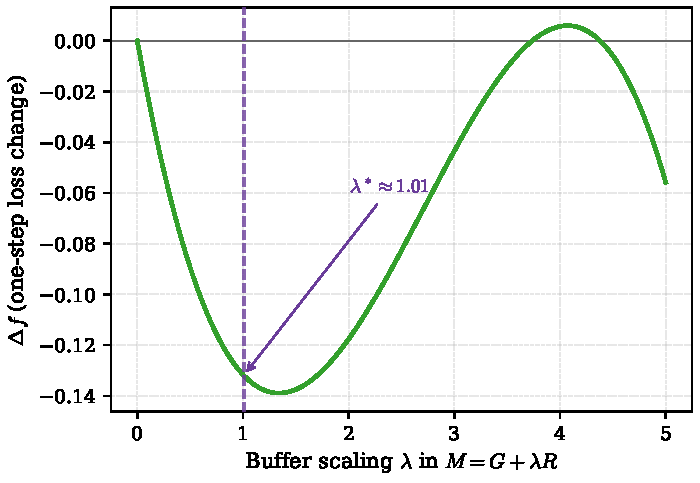
\includegraphics[width=0.55\linewidth]{figs/fig10_response.pdf}
\caption{Response surface at the $\beta = 0.3$ checkpoint (step 15{,}000). The fitted curve $\Delta f \approx -0.233\lambda + 0.116\lambda^2 - 0.014\lambda^3$ has its minimum at $\lambda^* \approx 1.01$.}
\label{fig:response}
\end{figure}

\begin{table}[h]
\centering
\caption{Response surface fits. The sweet spot $\lambda^*$ is stable at $\approx 1.0$ across checkpoints.}
\label{tab:response}
\begin{tabular}{lccc}
\toprule
\textbf{Checkpoint} & $a$ (linear) & $b$ (quadratic) & $\lambda^*$ \\
\midrule
$\beta{=}0.3$, step 5k & $-0.161$ & $0.083$ & 0.97 \\
$\beta{=}0.3$, step 15k & $-0.233$ & $0.116$ & 1.01 \\
$\beta{=}0.3$, step 25k & $-0.161$ & $0.084$ & 0.96 \\
$\beta{=}1.0$, step 15k & $-0.300$ & $0.144$ & 1.04 \\
\bottomrule
\end{tabular}
\end{table}

The linear coefficient $a$ is always negative (adding buffer signal reduces loss), and the quadratic coefficient $b$ is always positive (diminishing returns). The sweet spot $\lambda^* = -a/(2b) \approx 1.0$ is stable across training stages and $\beta$ values. The $\beta = 1.0$ checkpoint has a steeper curve ($|a| = 0.300$ vs 0.233), consistent with the hypothesis that models trained without buffer retention benefit more when buffer signal is introduced post hoc.

% =====================================================================
\section{Experiment 5: Controller Comparison}
\label{sec:controllers}
% =====================================================================

We compare several adaptive $\beta$ controllers against the flat $\beta = 0.3$ baseline on GPT-2 45M (WikiText-103, 30k steps):

\begin{itemize}[nosep]
    \item \textbf{PA-Dion:} $\beta_t = \beta_{\min} + (\beta_{\max} - \beta_{\min}) \cdot \sigma(s \cdot (\rho_{\mathrm{ema},t} - \tau))$, where $\rho_{\mathrm{ema},t}$ is the EMA of the global persistence $\rho_t$.
    \item \textbf{RNormDion:} $\beta_t = \mathrm{clamp}(0.5 + k_p \cdot (R_{\mathrm{ema},t} - \rho^*), \beta_{\min}, \beta_{\max})$, a proportional controller targeting $\norm{R_t}_F / \norm{G_t}_F \approx \rho^*$.
    \item \textbf{ReEntryDion:} Similar to RNormDion but targeting $\norm{P_{t+1} R_t}_F / \norm{G_t}_F$ instead of $\norm{R_t}_F / \norm{G_t}_F$.
\end{itemize}

\begin{figure}[h]
\centering
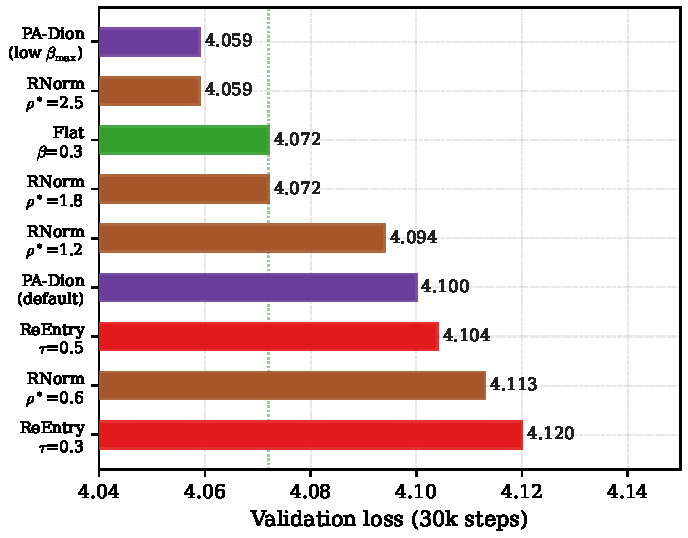
\includegraphics[width=0.6\linewidth]{figs/fig11_controllers.pdf}
\caption{Controller comparison. RNorm target${=}1.8$ exactly matches flat $\beta = 0.3$ (4.072), confirming $\norm{R}/\norm{G}$ as the operating variable.}
\label{fig:controllers}
\end{figure}

The key finding is that RNorm target${=}1.8$ produces the same result as flat $\beta = 0.3$ (both at 4.072). This confirms that the buffer-to-gradient ratio $\norm{R_t}_F / \norm{G_t}_F$ is the fundamental variable controlling error-feedback performance, and $\beta$ is one way to set it. Different control mechanisms (flat $\beta$, RNorm, PA-Dion) converge to the same result when they target the same operating point.

% =====================================================================
\section{Experiment 6: LLaMA 300M}
\label{sec:llama}
% =====================================================================

We evaluate Ada-Dion V3 at scale on a LLaMA-style model (308M parameters, 20 layers, 16 heads, 1024 hidden, SwiGLU FFN with inner dimension 2816, RoPE, RMSNorm, weight tying) trained on WikiText-103 with batch size 4, sequence length 1024.

Each optimizer undergoes a 4-point learning rate sweep (3k steps per LR) followed by a 15k-step run at the best LR.

\begin{figure}[h]
\centering
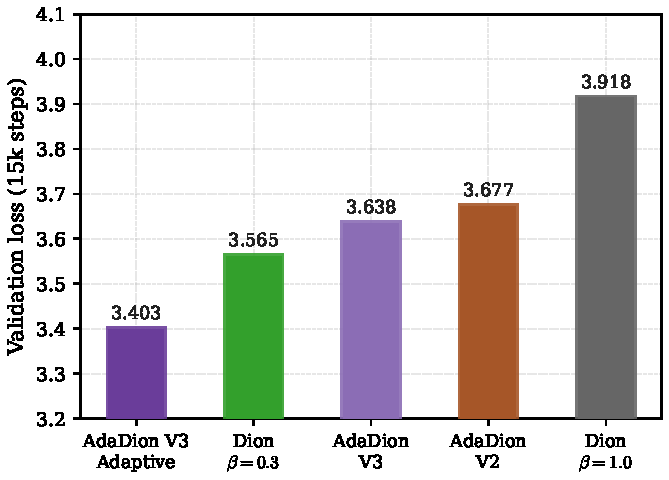
\includegraphics[width=0.6\linewidth]{figs/fig1_llama_main.pdf}
\caption{LLaMA 300M validation loss (15k steps, tuned LRs). V3 Adaptive achieves 3.403, compared to 3.565 for Dion $\beta{=}0.3$ and 3.918 for standard Dion.}
\label{fig:llama_main}
\end{figure}

\begin{table}[h]
\centering
\caption{LLaMA 300M results (WikiText-103, 15k steps).}
\label{tab:llama}
\begin{tabular}{lcccc}
\toprule
\textbf{Method} & \textbf{Val Loss} & \textbf{Comm (GB)} & \textbf{Tok/s} & \textbf{Mem (GB)} \\
\midrule
Muon & 3.277 & 30,828 & 4,703 & 25.0 \\
AdamW & 3.381 & 18,504 & 19,001 & 21.8 \\
\midrule
Ada-Dion V3 Adaptive & 3.403 & 11,998 & 4,792 & 14.1 \\
Dion $\beta{=}0.3$ & 3.565 & 1,456 & 14,056 & 22.0 \\
Ada-Dion V3 & 3.638 & 1,514 & 12,922 & 13.3 \\
Ada-Dion V2 & 3.677 & 6,826 & 10,595 & 13.3 \\
Dion $\beta{=}1.0$ & 3.918 & 1,456 & 14,153 & 22.0 \\
\bottomrule
\end{tabular}
\end{table}

\begin{figure}[h]
\centering
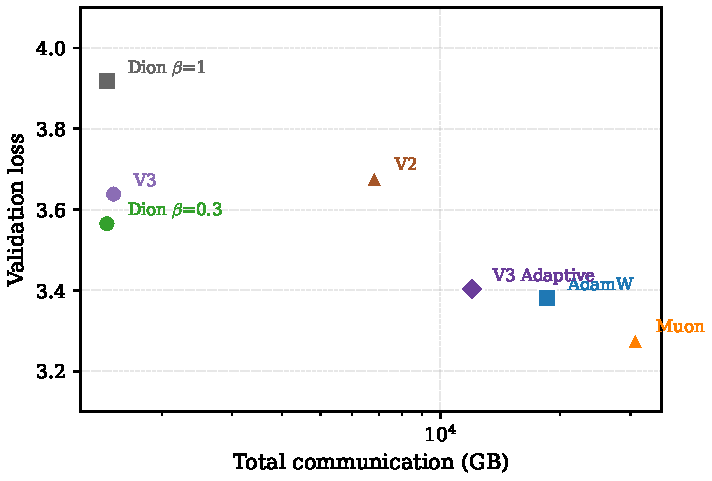
\includegraphics[width=0.6\linewidth]{figs/fig2_pareto.pdf}
\caption{Communication vs.\ validation loss trade-off for LLaMA 300M.}
\label{fig:pareto}
\end{figure}

Several observations are worth noting. The gap between $\beta = 0.3$ and $\beta = 1.0$ grows from 0.407 nats at 45M to 0.353 nats at 300M with a much lower absolute loss, suggesting the mechanism remains important at scale. V3 Adaptive (3.403) comes within 0.022 nats of AdamW (3.381). V3 without adaptive rank (3.638) uses only 1{,}514 GB of communication, comparable to standard Dion, while reducing loss by 0.280 nats relative to $\beta = 1.0$. The memory reduction (14.1 vs 22.0 GB) is a consequence of the buffer clamping and per-mode control preventing unbounded state growth.

% =====================================================================
\section{Experiment 7: Vision Benchmarks}
\label{sec:vision}
% =====================================================================

\begin{figure}[h]
\centering
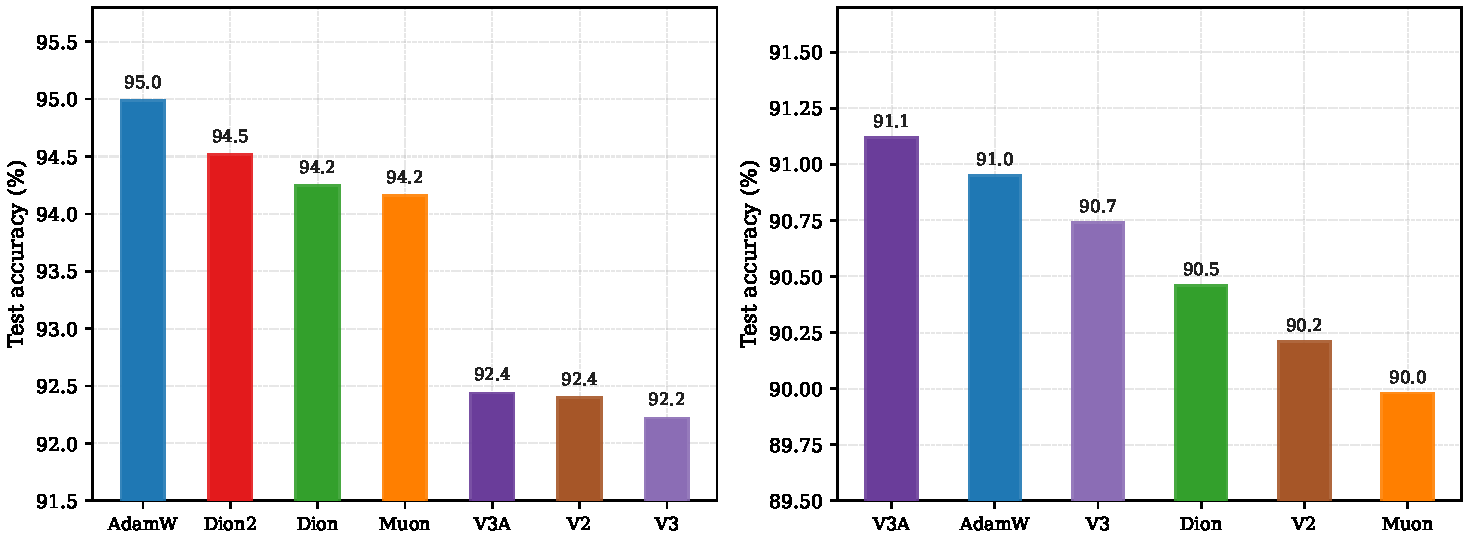
\includegraphics[width=0.9\linewidth]{figs/fig3_vision.pdf}
\caption{(Left) CIFAR-10 with ResNet-18, 100 epochs. (Right) FashionMNIST with 3-layer MLP (2048 hidden), 50 epochs.}
\label{fig:vision}
\end{figure}

\begin{table}[h]
\centering
\caption{Vision benchmark results.}
\label{tab:vision}
\begin{tabular}{llccc}
\toprule
\textbf{Dataset} & \textbf{Optimizer} & \textbf{Test Acc (\%)} & \textbf{Comm (GB)} & \textbf{Mem (GB)} \\
\midrule
\multirow{6}{*}{CIFAR-10} & AdamW & 94.99 & 1,743 & 0.83 \\
 & Dion2 & 94.52 & 1.42 & 0.83 \\
 & Dion & 94.25 & 1.42 & 0.83 \\
 & Muon & 94.16 & 1.60 & 0.83 \\
 & V3 Adaptive & 92.44 & 0.81 & 0.83 \\
 & V3 & 92.22 & 0.81 & 0.83 \\
\midrule
\multirow{6}{*}{FashionMNIST} & V3 Adaptive & 91.12 & 10.26 & 0.21 \\
 & AdamW & 90.95 & 272.40 & 0.13 \\
 & V3 & 90.74 & 21.71 & 0.21 \\
 & Dion & 90.46 & 25.02 & 0.20 \\
 & V2 & 90.21 & 26.13 & 0.13 \\
 & Muon & 89.98 & 544.79 & 0.37 \\
\bottomrule
\end{tabular}
\end{table}

On FashionMNIST, V3 Adaptive (91.12\%) exceeds AdamW (90.95\%) with $27\times$ less communication. On CIFAR-10, spectral optimizers trail AdamW by 2--3\%, which may reflect the mismatch between the spectral update (designed for linear layers) and convolutional layers (handled via AdamW in all spectral methods).

% =====================================================================
\section{Development Notes: Debugging at Scale}
\label{sec:autopsy}
% =====================================================================

V3 initially produced val loss $>$ 6.0 at 300M scale. A systematic ablation study running 7 variants of V3 (each isolating one component) for 500 steps with per-parameter diagnostics identified two bugs.

First, V3 applied the spectral update to the embedding matrix ($50{,}257 \times 1{,}024$), which is a vocabulary lookup table not amenable to low-rank optimization. Routing it to AdamW resolved the largest source of divergence.

Second, partial orthogonalization (ColNorm followed by one round of damped Gram-Schmidt), which reduces $\nu_t$ at 45M scale, increases $\nu_t$ from 3.0 to 5.0 at 300M scale because column norm ratios exceed 300. Reverting to pure ColNorm resolved the remaining instability.

The ablation methodology, which we describe here to benefit future optimizer development, works as follows: from the same model initialization and data order, run the working baseline (Dion $\beta{=}0.3$) and the broken optimizer (V3) side by side for a small number of steps, logging per-parameter $\norm{G}$, $\norm{R}$, $\norm{D}$, $\nu_t$, effective rank, and update magnitude at each step. Divergence between the two traces localizes the bug to a specific component.

% =====================================================================
\section{Discussion}
\label{sec:discussion}
% =====================================================================

\subsection{Summary of Findings}

\begin{enumerate}
    \item Buffer retention ($\beta < 1$) provides 0.4--0.5 nats improvement over $\beta = 1$ at zero additional compute cost. The benefit is consistent across ranks and scales.

    \item QR orthogonalization fails in practice at all ranks and scales tested. The theory's $\sqrt{r}$ rate improvement does not materialize because the spectral gap assumption ($\sigma_r / \sigma_{r+1}$ bounded away from 1) does not hold at rank 64 in LLM training. ColNorm is the only robust right-factor normalization across scales.

    \item Per-mode gradient persistence is heterogeneous by a factor of $28\times$, motivating per-mode $\beta_i$ control. Ada-Dion V3 implements this with a sigmoid controller.

    \item $\norm{R_t}_F / \norm{G_t}_F$ is the fundamental operating variable for error feedback. Different control mechanisms converge to the same result when targeting the same ratio.

    \item The response surface has a stable sweet spot at $\lambda^* \approx 1.0$ across training stages and configurations.
\end{enumerate}

\subsection{Coupling Between Geometry and Memory}

A recurring theme is that the right-factor normalization and the error-feedback mechanism are coupled, not independent. ColNorm produces tracking error $\hat{\epsilon}_t \approx 0.15$--$0.30$, which enables the implicit momentum mechanism that makes $\beta < 1$ effective. QR reduces tracking error to $\hat{\epsilon}_t \approx 0.007$, eliminating implicit momentum and rendering $\beta < 1$ ineffective. Partial orthogonalization (which reduces $\nu_t$ while maintaining moderate $\hat{\epsilon}_t$) works at 45M but becomes unstable at 300M when column norm ratios are large.

The convergence theory analyzes two extremes: $\nu_t = 1$ (QR) and $\nu_t = \sqrt{r}$ (worst-case ColNorm). Our experiments operate in the intermediate regime $1.5 \leq \nu_t \leq 3.5$, where the interplay between $\nu_t$, $\hat{\epsilon}_t$, and $\beta$ determines convergence. Extending the theory to this regime is an open problem.

\subsection{Limitations}

V3 Adaptive achieves the best loss at 300M but at 4{,}792 tok/s, which is $3\times$ slower than Dion (14{,}056 tok/s) due to adaptive rank overhead. This is an implementation efficiency issue, not a fundamental limitation, and can likely be addressed through better batching of the rank adaptation step.

All experiments use single-GPU training with simulated FSDP communication accounting. Multi-node distributed validation is needed to confirm the communication savings translate to wall-clock speedups.

The per-mode sigmoid controller uses fixed hyperparameters ($s = 10$, $\alpha = 0.95$) across all experiments. It is possible that task-specific tuning would further improve results.

\bibliographystyle{plain}
\bibliography{references}

\end{document}
